\documentclass[a4paper]{article}

\usepackage[T2A]{fontenc}
\usepackage[utf8]{inputenc}
\usepackage[russian]{babel}
\usepackage{graphicx}
\usepackage{float}
\usepackage{mathtools}
\usepackage{wrapfig}
\usepackage{amsfonts, amssymb, amsmath, latexsym}
\usepackage{nicefrac}
\usepackage{hhline}
\usepackage{multirow}
\usepackage[colorlinks=true,linkcolor=blue,citecolor=blue]{hyperref}       % hyperlinks
\usepackage{nicefrac}       % compact symbols for 1/2, etc.
\usepackage{nameref}
\usepackage{booktabs}       % professional-quality tables
\usepackage{algorithm}
\usepackage{algpseudocode}
\usepackage{xcolor, colortbl}
\usepackage{etoolbox}

% \graphicspath{ {./} }

\usepackage[verbose=true,letterpaper]{geometry}

\newgeometry{
    textheight=25cm,
    textwidth=18cm,
    top=2.5cm,
    headheight=12pt,
    headsep=10pt,
    footskip=1cm,
    marginparwidth=15pt
}

%\usepackage{showframe} 

\usepackage{epigraph}
\usepackage{amsmath,amsfonts,amssymb,amsthm,mathtools, mathrsfs}
\usepackage{amsthm}

\title{Работа 4.5.2 \\ Интерференция лазерного излучения}
\author{Шарапов Денис, Б05-005}
\date{}

\usepackage{fancyhdr}
\pagestyle{fancy}
\fancyhf{}
\rhead{Работа 4.5.2}
\lhead{}
\cfoot{\thepage}
\usepackage{subcaption}
\usepackage[font={small}]{caption}

\begin{document}

    \maketitle
    \tableofcontents
    \newpage
    
\section{Аннотация}

\noindent\textbf{Цель работы:} исследование видности интерференционной картины излучения гелий-неонового лазера и определение длины когерентности излучения. \smallskip
 
\noindent \textbf{В работе используются:} He-Ne-лазер, интерферометр Майкельсона с подвижным зеркалом, фотодиод с усилителем, осциллограф, поляроид, линейка.

\section{Теоретические сведения}

Типичная осциллограмма сигнала фотодиода приведена на рис. 1. По осциллограмме можно найти следующие величины: фоновую засветку (линия 0 — перекрыты оба пучка 1 и 2); интенсивность света каждого из пучков (линии 1 или 2 — перекрыт пучок 2 или 1); максимума и минимума интенсивности интерференционной картины (открыты оба пучка).

\begin{figure}[ht!]
    \centering
    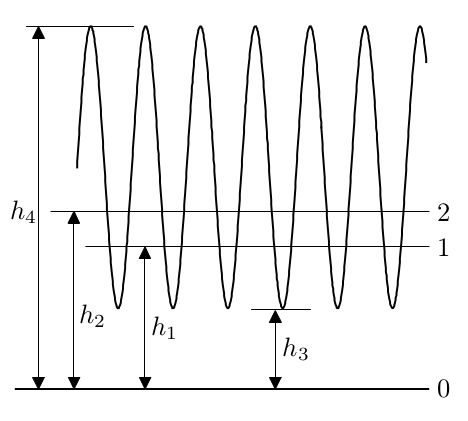
\includegraphics[width = 0.35\textwidth]{image/picture1.png}
    \caption{Осциллограмма сигналов с фотоида}
\end{figure}

\noindent Видность интерференционной картины рассчитывается по формуле $$V = \frac{h_4 - h_3}{h_4 + h_3}.$$

\section{Экспериментальная установка}

Для получения интерференционной картины используется интерферометр Майкельсона, смонтированный на вертикально стоящей массивной металлической плите. Схема установки приведена на рис. 1.

\begin{figure}[ht!]
    \centering
    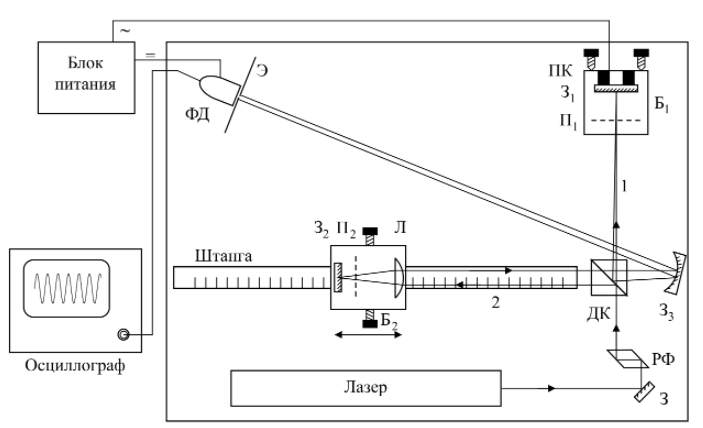
\includegraphics[width = 0.7\textwidth]{image/scheme.png}
    \caption{Схема установки. З, З$_1$, З$_2$, З$_3$ -- зеркала. П$_1$ и П$_2$ -- поляроиды. Б$_1$ и Б$_2$ -- блоки. ДК -- делительный кубик, РФ -- ромб Френеля. ФД -- фотодиод, Э -- экран, ПК -- пьезокерамика, Л -- линза}
\end{figure}

Источником света служит гелий-неоновый лазер (средняя длина волны $\lambda$ = 632,8 нм). Пучок лазерного излучения отражается от зеркала З и проходит призму полного внутреннего отражения РФ (ромб Френеля), которая превращает линейную поляризацию излучения в круговую. Если в установке используется лазер, излучающий неполяризованный свет, то ромб Френеля не нужен, но он и не мешает выполнению работы.
Далее лазерное излучение делится диагональной плоскостью делительного кубика ДК на два пучка.

Пучок 1 проходит поляроид П$_1$, отражается под небольшим углом от зеркала З$_1$, снова проходит поляроид П$_1$ и, частично отражаясь от диагональной плоскости делительного кубика, выходит из интерферометра, попадает на зеркало З$_3$ и далее на фотодиод ФД. Зеркало З$_1$ наклеено на пьезокерамику ПК, которая может осуществлять малые колебания зеркала вдоль направления распространения падающего пучка. Поляроид и зеркало с пьезокерамикой собраны в единый блок Б$_1$, который крепится к вертикально стоящей плите. В блоке Б$_1$ имеются юстировочные винты, которые позволяют регулировать угол наклона зеркала З$_1$. В установке предусмотрена возможность вращения поляроида П$_1$. Угол поворота отсчитывается по шкале, нанесённой на оправу
поляроида.

Пучок 2 проходит линзу Л, поляроид П$_2$, отражается от зеркала З$_2$, снова проходит поляроид П$_2$, линзу Л и делительный кубик, выходит из интерферометра, попадает на зеркало З$_3$ и далее на фотодиод ФД. Таким образом, от зеркала З$_3$ под небольшим углом друг к другу идут на фотодиод два пучка, прошедшие разные плечи интерферометра. Между ними происходит интерференция и образуются интерференционные полосы. Линза Л,
поляроид П$_2$ и зеркало З$_2$ собраны в единый блок Б$_2$. Зеркало З$_2$ установлено в фокальной плоскости линзы Л. Это сделано для того, чтобы падающий и выходящий из блока Б$_2$ пучки всегда были параллельны друг другу. Блок Б$_2$ может перемещаться вдоль пучка 2 по штанге, жёстко связанной с плитой интерферометра. Длина штанги 90 см. В установке предусмотрена возможность небольшого поперечного перемещения блока Б$_2$, что позволяет регулировать расстояние между падающим и выходящим из блока пучками. При измерениях блок Б$_2$ крепится к штанге при помощи двух винтов. Вдоль штанги нанесены деления через один сантиметр.

\section{Результаты измерений и обработка данных}

\subsection{Зависимость видности интерференционной картины от угла поворота поляроида}

Исследуем зависимость видности интерференционной картины от угла $\beta$ поворота поляроида П$_1$ при нулевой разности хода. Результаты занесём в таблицу 1. По таблице построим графики зависимостей $V_3(\cos{\beta})$ и $V_3(\cos^2{\beta})$ (рис. 3 и 4).

\begin{figure}[ht!]
    \centering
    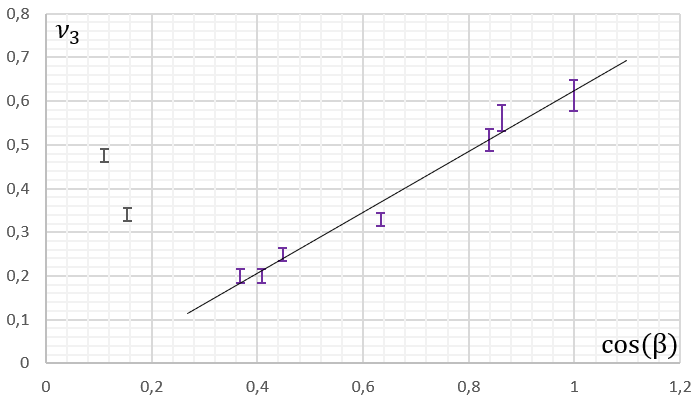
\includegraphics[width = 0.7\textwidth]{image/graph1.png}
    \caption{График зависимости видности интерференционной картины от угла поворота поляроида: случай 1}
\end{figure}

\begin{figure}[ht!]
    \centering
    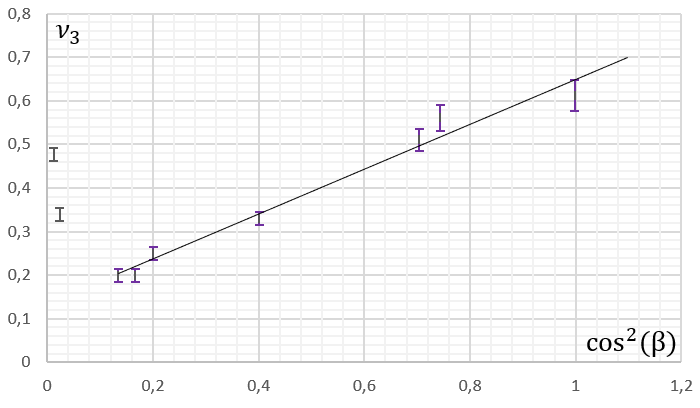
\includegraphics[width = 0.7\textwidth]{image/graph2.png}
    \caption{График зависимости видности интерференционной картины от угла поворота поляроида: случай 2}
\end{figure}

\subsection{Зависимость видности от разности хода между пучками}

Исследуем зависимость видности от разности хода между пучками. Для этого установим поляроид П$_1$ в положение, в котором интерференционная картина видна наиболее чётко. Передвигая блок Б$_2$, найдём зависимость величин  $h_1, h_2, h_3, h_4$ от координаты $x$ блока Б$_2$. Результаты внесём в таблицу 2. По ней построим график зависимости $\nu_2(x)$.

\begin{figure}[ht!]
    \centering
    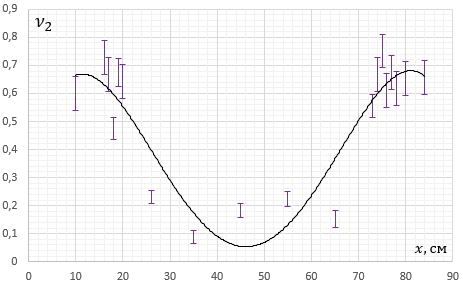
\includegraphics[width = 0.7\textwidth]{image/graph3.png}
    \caption{График зависимости видности интерференционной картины от разности хода между пучками}
\end{figure}

\noindent По графику определим значение $L$ --- расстояние между зеркалами оптического резонатора лазера: $$L \approx 46 \pm 0,3 \; \text{см}.$$

\noindent Рассчитаем межмодовое расстояние $\Delta\nu$: $$\Delta\nu \approx (3,26 \pm 0,06) \cdot 10^{8} \; \text{Гц}.$$

\noindent Рассчитаем геометрическую задержку $l_{1/2}$, при которой видность падает вдвое: $$l_{1/2} \approx 55,2 \;\text{см}.$$

\noindent Теперь определим число мод $n$: $$n = 2 \pm 1.$$

\section{Вывод}

В работе исследовалась видность интерференционной картины излучения гелий-неонового лазера. На графиках, изображенных на рис. 3 и 4, представлена зависимость видности интерференционной картины от угла поворота поляроида. Видно, что точки на рис. 4 <<ложатся>> на прямую лучше, чем точки на рис. 3. Возможно, это может быть связано с тем, что вектор \textbf{E} хаотически меняет своё направление (находясь при этом в плоскости поляризации, т. к. она предполагается линейной). Из графика, изображённого на рис. 5, можно найти число мод (аналитически и геометрически). Из геометрической интерпретации находим число мод $n = 3$. При этом аналитическая интерпретация с точностью до погрешности даёт тот же результат $n = 2 \pm 1$.

\section{Приложение: таблицы}

\begin{table}[!ht]
    \centering
    \caption{Зависимость видности интерференционной картины от угла поворота поляроида}
    \begin{tabular}{|c|c|c|c|c|c|c|c|c|c|c|}
    \hline
    $\beta$ & $h_1$, дел & $h_2$, дел & $h_3$, дел & $h_4$, дел & $\delta$ & $\nu$ & $\nu_1$ & $\nu_3$ & $\cos(\beta)$ & $\cos^2(\beta)$ \\ \hline
    10                 & 1,2   & 0,8   & 1,0   & 3,0   & 1,50     & 0,50  & 0,98    & 3,00    & 0,84          & 0,70            \\ \hline
    20                 & 1,2   & 0,4   & 1,0   & 2,6   & 3,00     & 0,44  & 0,87    & 0,20    & 0,41          & 0,17            \\ \hline
    30                 & 1,2   & 0,4   & 1,2   & 2,2   & 3,00     & 0,29  & 0,87    & 10,20   & 0,15          & 0,02            \\ \hline
    40                 & 1,2   & 0,2   & 1,4   & 1,6   & 6,00     & 0,07  & 0,70    & 90,00   & 0,67          & 0,44            \\ \hline
    60                 & 1,2   & 0,2   & 1,2   & 1,4   & 6,00     & 0,08  & 0,70    & 78,00   & 0,95          & 0,91            \\ \hline
    60                 & 1,2   & 0,2   & 1,2   & 1,6   & 6,00     & 0,14  & 0,70    & 42,00   & 0,95          & 0,90            \\ \hline
    70                 & 1,2   & 0,4   & 1,0   & 1,8   & 3,00     & 0,29  & 0,87    & 10,50   & 0,63          & 0,40            \\ \hline
    80                 & 1,2   & 0,2   & 1,0   & 2,0   & 6,00     & 0,33  & 0,70    & 18,00   & 0,11          & 0,01            \\ \hline
    90                 & 1,2   & 0,4   & 0,8   & 2,2   & 3,00     & 0,47  & 0,87    & 0,25    & 0,45          & 0,20            \\ \hline
    100                & 1,2   & 0,6   & 0,8   & 2,6   & 2,00     & 0,53  & 0,94    & 3,78    & 0,86          & 0,74            \\ \hline
    110                & 1,2   & 0,8   & 0,8   & 3,2   & 1,50     & 0,60  & 0,98    & 2,50    & 0,99          & 0,98            \\ \hline
    130                & 1,2   & 0,8   & 0,6   & 3,0   & 1,50     & 0,67  & 0,98    & 0,20    & 0,36          & 0,13            \\ \hline
    \end{tabular}
    \end{table}

    \begin{table}[!ht]
        \centering
        \caption{Зависимость видности от разности хода между пучками}
        \begin{tabular}{|c|c|c|c|c|c|c|c|c|}
        \hline
        $x$, см & $h_1$, дел & $h_2$, дел & $h_3$, дел & $h_4$, дел & $\delta$ & $V$  & $V_1$ & $V_2$ \\ \hline
        16  & 1,40  & 0,60  & 0,60  & 3,0   & 2,33     & 0,67 & 0,92  & 0,73  \\ \hline
        18  & 2,00  & 0,80  & 1,20  & 3,0   & 2,50     & 0,43 & 0,90  & 0,47  \\ \hline
        20  & 0,60  & 0,80  & 0,40  & 1,8   & 0,75     & 0,64 & 0,99  & 0,64  \\ \hline
        17  & 0,60  & 0,60  & 0,40  & 2,0   & 1,00     & 0,67 & 1,00  & 0,67  \\ \hline
        19  & 0,60  & 0,80  & 0,40  & 2,0   & 0,75     & 0,67 & 0,99  & 0,67  \\ \hline
        26  & 0,60  & 0,60  & 1,00  & 1,6   & 1,00     & 0,23 & 1,00  & 0,23  \\ \hline
        35  & 2,20  & 0,80  & 2,40  & 2,8   & 2,75     & 0,08 & 0,88  & 0,09  \\ \hline
        45  & 1,80  & 0,60  & 1,60  & 2,2   & 3,00     & 0,16 & 0,87  & 0,18  \\ \hline
        55  & 1,00  & 0,20  & 1,00  & 1,4   & 5,00     & 0,17 & 0,75  & 0,22  \\ \hline
        65  & 0,40  & 0,20  & 1,20  & 1,6   & 2,00     & 0,14 & 0,94  & 0,15  \\ \hline
        74  & 2,80  & 0,80  & 1,20  & 4,2   & 3,50     & 0,56 & 0,83  & 0,67  \\ \hline
        75  & 2,80  & 0,80  & 1,20  & 5,2   & 3,50     & 0,63 & 0,83  & 0,75  \\ \hline
        \end{tabular}
        \end{table}


\end{document}